\newif \iftheory 

\theorytrue %\theoryfalse

\newif \ifblind

\blindtrue \blindfalse

\newcommand{\eli}[1]{\textcolor{blue}{[Eli: #1]}}
\newcommand{\meg}[1]{\textcolor{red}{[Megumi: #1]}}
\newcommand{\hannah}[1]{\textcolor{magenta}{[Hannah: #1]}}


% ~~~~~ Modify inside here ~~~~~%
\newcommand{\authorlist}{
% Author 1
Megumi Ando\iftheory\thanks{Computer Science Department, Tufts University, {\tt mando@cs.tufts.edu}}\fi
\and 
% Author 2
Anna Lysyanskaya\iftheory\thanks{Computer Science Department, Brown University, {\tt anna@cs.brown.edu}}\fi
\and 
% Author 3
Hannah Marsh\iftheory\thanks{Computer Science Department, Tufts University, {\tt hannah@cs.tufts.edu}}\fi
\and
% Author 3
Eli Upfal\iftheory\thanks{Computer Science Department, Brown University, {\tt eli\_upfal@brown.edu}}\fi
}

\newcommand{\institutelist}{}


\newcommand{\titlelist}{\iftheory\begin{bf}\fi
% title
Onion Routing on Sparse Distributed Networks
\iftheory\end{bf}\fi}

% Path to stylefiles
\newcommand{\pathstyles}{./stylefiles}

% Path to preambles
\newcommand{\pathpreambles}{./preambles}

% Path to bibfiles
\newcommand{\pathbibs}{./bibfiles}

% ~~~~~ Modify inside here ~~~~~%


\iftheory
% PLAIN ARTICLE
\documentclass[11pt]{article}

% LNCS (DEFAULT)
\else
%\documentclass[envcountsame, 10pt]{\pathstyles/llncs}
\documentclass[runningheads,a4paper]{llncs}
\ifblind 
\institute{}
\else
\institute{\institutelist}
\fi
\fi

\ifblind 
\author{}
\else
\author{\authorlist} 
\fi
\pagestyle{plain}

\title{\titlelist}

% PREAMBLE
% PREAMBLE
\usepackage[utf8]{inputenc}
\usepackage{amsfonts}
\usepackage{amssymb}
\usepackage{circuitikz}
\usepackage{cite}

\usepackage{xcolor}
\usepackage[
	n,
	operators,
	advantage,
	sets,
	adversary,
	landau,
	probability,
	notions,	
	logic,
	ff,
	mm,
	primitives,
	events,
	complexity,
	asymptotics,
	keys]{cryptocode}
\usepackage{enumitem}
\setlist{nosep}
\usepackage[hidelinks]{hyperref}
%\usepackage{todonotes}

\usepackage{lscape}
\usepackage{mathtools}

% MACROS

% ~~ General

%\DeclareMathOperator*{\argmax}{arg\,max}
%\DeclareMathOperator*{\argmin}{arg\,min}

\renewcommand{\secpar}{\lambda}
\renewcommand{\secparam}{1^\lambda}


% ~~ Formatting
\definecolor{hybrid}{HTML}{0076BA}

\usepackage{caption} 
\captionsetup[table]{skip=10pt}


% ~~~ Begin document ~~~ %
\begin{document}

\maketitle
\iftheory
\thispagestyle{empty}
\fi

% ABSTRACT
\vspace{-8mm}
\begin{abstract}
A network adversary is an entity with complete visibility of all traffic flowing through a distributed network. Even when a message’s content is encrypted, a network adversary can analyze traffic patterns to infer who is communicating with whom—a form of surveillance that can be exploited for control and influence. Anonymous communication protocols defend against this by introducing uncertainty in how messages traverse the network. \textit{Onion routing} is a widely adopted approach that achieves anonymity by encrypting messages in layers and relaying them through multiple intermediaries. Prior work by Ando, Lysyanskaya, and Upfal [ICALP 2018] showed that when intermediate nodes are selected uniformly at random in a complete-graph topology, the variation distance between a network adversary’s view of any two communication patterns decays faster than any inverse polynomial in the security parameter. This strong, provable definition of anonymity, known as \textit{statistical privacy}, holds when onions are batch-processed with a polylogarithmic number of other onions for a polylogarithmic number of rounds (in the security parameter).

We extend this result to sparse networks modeled as $r$-regular expander graphs, where each server connects to only a small constant ($r > 2$) number of neighbors. By routing onions via independent, fixed-length random walks, we show that statistical privacy can still be achieved against a network adversary, with both server load and path length remaining polylogarithmic in the security parameter. This result demonstrates that practical and provably secure communication is possible even in sparsely connected distributed networks.

\iftheory
\vfill
%\noindent\textbf{Keywords:} 
%Keyword, 
%keyword, 
%keyword.
\fi
\end{abstract}
 

% ~~~ BODY ~~~ %
\iftheory
\newpage
\thispagestyle{empty}
\newpage
\setcounter{page}{1}
\fi

\newcommand{\parties}{\mathsf{Parties}}
\newcommand{\keygen}{\mathsf{KeyGen}}
\newcommand{\formonion}{\mathsf{FormOnion}}
\newcommand{\proconion}{\mathsf{PeelOnion}}
\newcommand{\proconionhelper}{\mathsf{PeelOnionHelper}}
\newcommand{\bruiseonion}{\mathsf{BruiseOnion}}
\newcommand{\polylog}{\mathsf{polylog}}
\newcommand{\early}{\mathsf{early}}
\newcommand{\late}{\mathsf{late}}
\newcommand{\recipient}{\mathsf{Recipient}}
\newcommand{\Bad}{\mathsf{Bad}}

\section{Introduction}

Protecting user privacy in communication is a growing challenge in modern networks. Anonymous communication channels are essential for preventing adversaries from linking users to their activities, whether it's for online privacy, whistleblowing, or secure voting. One well-known method for achieving anonymous communication is \textit{onion routing}, where messages are wrapped in layers of encryption and routed through a series of intermediaries before reaching the intended recipient. Each intermediary decrypts a single layer, revealing only the next node in the chain and the ciphertext to forward. 

Onion routing is widely adopted due to its simplicity and ability to tolerate failures in a subset of nodes. Systems like Tor \cite{tor}, which implement onion routing, are used by millions of people daily to protect their online activities. However, despite its widespread use, the security guarantees of onion routing are not fully understood, especially in the face of powerful adversaries.

Previous work, such as the protocol $\Pi_p$ introduced in~\cite{ICALP:AndLysUpf18}, shows that \textit{statistical privacy} can be achieved against a passive adversary if the intermediaries in the mixnet are chosen uniformly at random from all available nodes in a fully connected network. However, this approach relies on a complete graph, where every node can communicate directly with every other node, leading to a quadratic increase in the number of network edges as the system scales to accommodate more mixnodes. Thus the fully connected mixnet is inefficient for large systems.

We present the design and evaluation of $\Pi_x$, a new protocol that aims to provide similar levels of anonymity while requiring significantly fewer network edges. Instead of relying on a fully connected mixnet, $\Pi_x$ assumes an \textit{expander} topology, a class of sparse graphs that maintain strong connectivity even with very few edges. In our approach, each mix-node has a probability distribution based on its connections to a fixed number of other nodes, from which clients select the next hop in their routing path. We demonstrate that, by configuring these distributions to approximate an expander graph, $\Pi_x$ can provide the same anonymity guarantees as a fully connected network but with only $O(n)$ edges.

We demonstrate that expander graphs can be a practical foundation for large-scale anonymous communication systems, providing a balance between efficiency and privacy.

\subsection{Progression of Goals}

In our exploration of onion routing protocols on an expander topology, we begin with the foundational settings introduced in~\cite{ICALP:AndLysUpf18}, which assumes a synchronous communication model where all messages are delivered within fixed rounds. The goal is to achieve statistical privacy against the network and passive adversaries, and differential privacy against the active adversary. We first aim to generalize these results to an expander topology. 

However, a practical challenge of this adaption is enabling efficient onion formation for senders without requiring full knowledge of the network topology, which may change between and even within a single execution of the protocol. In the first results of this paper, clients need to download and maintain the global network structure to select routing paths. However, this becomes impractical as the network scales. To address these issues, we propose a novel protocol extension: wrapping onions. In this approach, the client forms an initial onion with partial routing information and sends it to the first intermediary node. This node peels the first layer to reveal the next destination node, but because the graph is an expander, there may not be a direct link. Instead, the intermediary node must create a detour path to the next hop, wrapping the onion in additional layers, and forwarding it onward. By delegating some of the routing decisions to intermediary nodes, the protocol significantly reduces the burden on clients, as they no longer need to download or maintain the entire network topology. This wrapping mechanism also aligns well with the expander graph's natural properties, where efficient routing can be achieved with localized knowledge.

Another advantage of this approach becomes evident when the network experiences churn, where nodes and edges are dynamically added or removed during execution. In a static topology, an onion formed at the start of the protocol could potentially die at some point if a node goes offline. However, in the wrapping onions protocol, the responsibility for routing dynamically shifts to intermediary nodes, which are better positioned to adapt to local changes in the network. This makes the protocol inherently more robust to churn, as local routing decisions can reflect the current network state.

In summary, our progression starts by generalizing the provable guarantees of $\Pi_p$ and $\Pi_a$ to an expander graph topology, then we build on this foundation with the wrapping onions protocol, which enhances scalability by minimizing client-side network requirements and improves computational efficiency.


\section{Definitions}

\subsection{Security Parameter}

The security parameter\footnote{It is worth noting that ``$\lambda$'' is also commonly used to denote eigenvalues (of a graph's adjacency matrix). To avoid confusion, we will explicitly specify whenever $\lambda$ represents something other than the security parameter.}, $\lambda \in \mathbb{N}$, is a tunable input that quantifies a system's level of security. It can be adjusted to achieve various trade-offs (e.g., privacy vs. latency), since many system parameters and metrics are bound asymptotically by functions of $\lambda$. 

A function $f : \mathbb{N} \rightarrow \mathbb{R}$ is negligible in $\lambda$, written $f(\lambda) = \negl$, if for every polynomial~$p(\cdot)$ and all sufficiently large $\lambda$, 
$$
f(\lambda) < \frac{1}{p(\lambda)}.
$$
An event occurs with overwhelming probability if it is the complement of an event with probability negligible in $\lambda$. We say that two families of distributions~$\{D_{0, \lambda}\}_{\lambda \in\mathbb{N}}$ and $\{D_{1, \lambda}\}_{\lambda \in\mathbb{N}}$ are statistically close if the statistical distance between $D_{0, \lambda}$ and $D_{1, \lambda}$ is negligible in $\lambda$~\footnote{When the security parameter is clear by context, we abbreviate this notion by $D_0 \approx_s D_1$.}.

\subsection{Network and Participants}

Our setup requires two distinct roles: $N$ clients (users), who wish to send private messages to other clients, and a network of $n$ relays (mixnodes) that serve as intermediaries to unlink sender-receiver pairs. While each client has a direct connection to every relay, we model the mixnet of relays as an $r$-regular, $\beta$-expander graph, where all relays are assumed to be synchronized. In our definitions, $N$ is polynomially bounded by the security parameter $\lambda$. Additionally, the size of the mixnet, $n$, is bounded by: $O\left(\frac{N}{log^2 \lambda}\right)$. 

Each input to a protocol $\Pi$ is represented as an $N$-dimensional vector. When the protocol is executed on an input $\sigma = (\sigma_1, \dots, \sigma_N)$, each $\sigma_i$ consists of a collection of properly formed message pairs. A message pair $(m,j) \in \sigma_i$ represents user $i$'s intention to send message $m$ to user $j$. Let $\mathcal{M}$ denote the (bounded) message space. Then $(m,j)$ is considered properly formed if $m \in \mathcal{M}$ and $j \in [N]$. 

Let $\mathcal{M}(\sigma)$ represent the set of all messages in $\sigma$. It is defined as the multiset of all message pairs across all users' inputs, given by

$$
\mathcal{M}(\sigma_1, \dots, \sigma_N) = \bigcup_{i=1}^{N} \{ (m,j) \in \sigma_i \}.
$$

\subsection{Threat Model}

Let $\Pi$ be a protocol, and let $\sigma$ be a vector of inputs to $\Pi$. Given an adversary $\mathcal{A}$, the view $\mathsf{V}^{\Pi,\mathcal{A}}(\sigma)$ of $\mathcal{A}$ consists of all the information observable by the adversary while participating in $\Pi$ on input $\sigma$, possibly with additional randomness used by the adversary to make its decisions. Given an adversary $\mathcal{A}$, the output $\mathsf{O}^{\Pi,\mathcal{A}}(\sigma) = (\mathsf{O}^{\Pi,\mathcal{A}}_1(\sigma), \dots, \mathsf{O}^{\Pi,\mathcal{A}}_N(\sigma))$ of $\Pi$ on input $\sigma$ is a vector of outputs for the $N$ parties.\\\\
We consider the following standard adversary models, listed in increasing order of capability:\\
\begin{itemize}
    \item \textbf{Network adversary.} A network adversary can observe the bits flowing over every link in the network. If data is encrypted in an idealized scenario, the only information that a network adversary has is the \textit{volume} of traffic flowing over edges in the network.)\\
    
    \item \textbf{Passive adversary.} In addition to the capabilities of a network adversary, a passive adversary can monitor the internal states and operations of a constant fraction of the relays. The adversary selects which relays to monitor non-adaptively, meaning the choice is made before the protocol begins and remains fixed throughout execution. Importantly, we assume the passive adversary has full knowledge of the network topology to inform their selection of whom to monitor.\\
    
    \item \textbf{Active adversary.} In addition to the capabilities of a passive adversary, an active adversary can corrupt the behavior of a constant fraction of the relays. While the selection of whom to corrupt remains non-adaptive (and may be informed by the network topology), the behavior of corrupted parties can be altered on the fly. This includes deviating arbitrarily from the protocol (e.g., dropping, delaying, or repeating onions). \\
\end{itemize}

\subsection{Privacy Definitions}

We define the security of a communications protocol as the difficulty for the adversary to infer who is communicating with whom (beyond what is leaked from captured messages). Below, we introduce two flavors of security notions. We will show that our constructions achieve either statistical privacy or $(\epsilon,\delta)$-differential privacy~\cite{TCC:DMNS06} in the idealized encryption setting.\\

\begin{definition} [Statistical privacy] \label{def:statistical-privacy}
    Let $\Sigma^*$ be the input set consisting of every input of the form
    $$
    \sigma = \{(m_1, \pi(1)), \dots, (m_N, \pi(N))\},
    $$
    where $m_1, \dots, m_N \in \mathcal{M}$ and $\pi : [N] \rightarrow [N]$ is any permutation function over the set $[N]$. A communications protocol $\Pi$ is statistically private from the adversaries in the class $\mathcal{A}$ if, for all $\mathcal{A} \in \mathcal{A}$ and for all $\sigma_0, \sigma_1 \in \Sigma^*$ that differ only on the honest parties' inputs and outputs, the adversary's views $\mathsf{V}^{\Pi,\mathcal{A}}(\sigma_0)$ and $\mathsf{V}^{\Pi,\mathcal{A}}(\sigma_1)$ are statistically indistinguishable, i.e.,
    $$
    \Delta(\mathsf{V}^{\Pi,\mathcal{A}}(\sigma_0), \mathsf{V}^{\Pi,\mathcal{A}}(\sigma_1)) = \mathsf{negl}(\lambda),
    $$
    where $\lambda \in \mathbb{N}$ denotes the security parameter, and $\Delta(\cdot, \cdot)$ denotes the statistical distance (i.e., the total variation distance). Protocol $\Pi$ is perfectly secure if the statistical distance is 0.
\end{definition}

\begin{definition} [Distance between inputs] \label{def:distance-between-inputs} 
    The distance between two inputs $\sigma_0 = (\sigma_1, \dots, \sigma_N)$ and $\sigma_1 = (\sigma_1', \dots, \sigma_N')$, denoted $d(\sigma_0, \sigma_1)$, is given by
    $$
    d(\sigma_0, \sigma_1) \overset{\Delta}{=} \sum_{i=1}^{N} |\sigma_{i} \vartriangle \sigma_{i}'|,
    $$
    where $\vartriangle$ represents the symmetric difference between $\sigma_{i}$ and $\sigma_{i}'$.\\
\end{definition}

\begin{definition} [Neighboring inputs] \label{def:neighboring-inputs} 
    Two inputs $\sigma_0$ and $\sigma_1$ are neighboring if 
    $$
    d(\sigma_0, \sigma_1) \leq 1.
    $$\\
\end{definition}

\begin{definition} [$(\epsilon, \delta)$-DP~\cite{TCC:DMNS06}] \label{def:dp}
    A communication protocol $\Pi$ is $(\epsilon, \delta)$-differentially private if for every adversary $\adv$ and every pair of neighboring inputs $\sigma_0$ and $\sigma_1$ and every set $\mathcal{V}$ of adversarial views, 
    $$
    \prob{\mathsf{View}^{\Pi, \adv}(\sigma_0) \in \mathcal{V}} \le e^\epsilon \prob{\mathsf{View}^{\Pi, \adv}(\sigma_1) \in \mathcal{V}} + \delta .
    $$
    
    While differential privacy is defined with respect to neighboring inputs, it also provides (albeit weaker) guarantees for non-neighboring inputs; it is known that the security parameters degrade proportionally with the distance between the inputs~\cite{TCC:DMNS06}.

    We say that $\Pi$ is computationally $(\epsilon,\delta)$-differentially private~\cite{C:MPRV09} if the above bound holds for all polynomially bounded adversaries.\\
\end{definition} 

\subsection{Performance Metrics}

\begin{definition} [Correctness] \label{def:correctness}
    We define correctness with respect to passive adversaries since message delivery cannot be guaranteed in the presence of an active adversary.
    \eli{we need appropriate definition for active adversary}\\
    
    A communications protocol $\Pi$ is said to be correct on an input $\sigma \in \Sigma$ if for any passive adversary $\mathcal{A}$, and for every recipient $j \in [N]$, the output $\mathsf{O}^{\Pi, \mathcal{A}}_j(\sigma)$ corresponds to the multiset of all messages for recipient $j$ in the input vector $\sigma$. That is,
    $$
    \mathsf{O}^{\Pi, \mathcal{A}}_j(\sigma) = \{m \mid (m, j) \in \mathcal{M}(\sigma)\},
    $$
    where $\mathcal{M}(\sigma)$ denotes the multiset of all messages in $\sigma$. \\
\end{definition}

\begin{definition} [Communication complexity blow-up] \label{def:ccb}
    The communication complexity blow-up of an OR protocol $\Pi$ is defined with respect to an input vector $\sigma$ and an adversary $\mathcal{A}$. 
    
    Denoted $\gamma^{\Pi, \mathcal{A}}(\sigma)$, it is the expected ratio between the total number $\Gamma^{\Pi, \mathcal{A}}(\sigma)$ of onions transmitted in protocol $\Pi$ and the total number $\mathcal{M}(\sigma)$ of messages in the input vector. That is,
    $$
    \gamma^{\Pi, \mathcal{A}}(\sigma) \overset{\Delta}{=} \mathbb{E} \left[ \frac{\Gamma^{\Pi, \mathcal{A}}(\sigma)}{|\mathcal{M}(\sigma)|} \right].
    $$

    $\gamma^{\Pi, \mathcal{A}}(\sigma)$ essentially measures how many more onion transmissions are required by the protocol, compared with transmitting the messages in onions directly from the senders to the recipients (without passing through intermediaries). We assume that every message $m \in \mathcal{M}$ in the message space $\mathcal{M}$ “fits” into a single onion. The communication complexity is measured in unit onions, which is appropriate when the parties pass primarily onions to each other.\\
\end{definition}

\begin{definition} [Server load] \label{def:serverload}
    The server load of an OR protocol $\Pi$ is defined with respect to an input vector $\sigma$ and an adversary $\mathcal{A}$. It is the expected number of onions processed by a single party in a round.\\
\end{definition}

\begin{definition} [Latency] \label{def:latency}
    The latency of an OR protocol $\Pi$ is defined with respect to an input vector $\sigma$ and an adversary $\mathcal{A}$. It is the expected number of rounds in a protocol execution.
    
    Protocols with having low (i.e., polynomial in the security parameter) server load, low communication complexity blow-up, and low latency are considered efficient OR protocols.\\
\end{definition}

\newpage

\subsection{Properties of Expander Graphs}

Expander graphs are a class of sparse graphs where any subset of its vertices remains well-connected to the rest of the graph, making them particularly useful in the design of network protocols.

\begin{definition} [$\beta$-expander] \label{def:beta-expander} ~\cite[Def. 1]{10.1007/3-540-49543-6_1}
    Formally, a graph $G = (V, E)$ is called a $\beta$-expander if, for every subset of vertices $S \subset V$ where $|S| \leq |V|/2$, the number of edges leaving $S$ (denoted by $\texttt{out}(S)$) satisfies:
    
    $$
    |\texttt{out}(S)| \geq \beta \cdot |S|.
    $$
    
    In other words, the number of edges connecting $S$ to its complement $V \setminus S$ is proportional to the size of $S$, so that that even small subsets of the graph are well-connected, as visualized in Fig.~\ref{fig:beta-expander}\\

    \begin{figure}
        \centering
        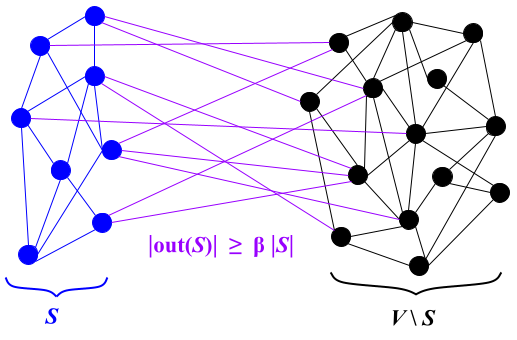
\includegraphics[width=0.5\textwidth]{template/figures/Expander graph.png}
        \caption{A graph $G = (V, E)$ is said to be a $\beta$-expander if the number of edges connecting any minority subset of vertices $S \subset V$ to its complement $V \setminus S$, denoted $|\texttt{out}(S)|$, is at least $\beta |S|$.}
        \label{fig:beta-expander}
    \end{figure}

\end{definition}

\begin{definition} [$\lambda$-absolute eiganvalue expander] \label{def:eiganvalue-expander}
     An $r$-regular graph $G = (V, E)$ is called a $\lambda$-absolute eiganvalue expander if, $|\lambda_2|,|\lambda_3|,...,|\lambda_n| \leq \lambda$. Here, $|\lambda_1| \geq |\lambda_2| \geq ... \geq |\lambda_n|$ are the eiganvalues of the adjacency matrix $A$ of $G$.\\

     In fact, iff $G$ is an $r$-regular $\beta$-expander, for some constant $\beta$, then it is also a $\lambda$-absolute eiganvalue expander where $\lambda = r - \frac{\beta^2}{2r}$ (from \textit{Cheeger's inequality}).
\end{definition}

\subsubsection{Random Walks} 
    
A \textit{random walk} on a graph is a process where, starting from an initial node, a ``walker'' moves to a neighboring node at each step according to some probability distribution over the neighbors of the current node. 

\begin{definition} [Simple random walk] \label{def:simp-random-walk}
    In a \textit{simple random walk} on a graph $G = (V, E)$, the walker starts at some vertex $v_0 \in V$. Let $\Gamma(v)$ denote the set of neighbors for each vertex $v \in V$. At each time step, the walker moves to a randomly chosen neighbor of the current vertex, where each neighbor is selected with equal probability. More formally, let $X_t$ denote the position of the walker at time $t$. The transition probability from vertex $v$ to vertex $u$ is given by:
    
    $$
    P(X_{t+1} = u \mid X_t = v) =
    \begin{cases}
    \frac{1}{|\Gamma(v)|} & \text{if } (v, u) \in E, \\
    0 & \text{otherwise}.
    \end{cases}
    $$
    
    Thus, at each step, the walker moves to one of the neighbors of the current vertex with equal probability.
\end{definition}

An important property is that a random walk on an expander graph rapidly converges to a uniform distribution, meaning that after a polylog number of steps (see Definition~\ref{def:bound-prob-distribution}), the probability of being at any given vertex becomes nearly uniform, regardless of the starting point.

\begin{definition} [Stationary distribution] \label{stationary-distribution}
    The \textit{stationary distribution} of a random walk is a probability distribution over the vertices such that if the walker is distributed according to this distribution at some time $t$, it will have the same distribution at time $t+1$. For a connected, non-bipartite graph, the random walk converges to a unique stationary distribution, and for regular graphs, this stationary distribution is uniform over all vertices.
\end{definition}

The rate of convergence to this stationary distribution in an expander graph is closely tied to the \textit{second-largest eigenvalue} of their adjacency matrix. 

\begin{definition} [Second-largest eigenvalue] \label{def:second-largest-eig}
    Let $\lambda_1 \geq \lambda_2 \geq \cdots \geq \lambda_n$ be the eigenvalues of the adjacency matrix of a $r$-regular graph. The largest eigenvalue $\lambda_1$ is equal to $r$, and the second-largest eigenvalue $\lambda_2$ (or the spectral gap $\lambda_1 - \lambda_2$) determines how quickly the random walk on the graph mixes. Specifically, the mixing time is inversely proportional to the spectral gap. A smaller value of $\lambda_2$ indicates faster mixing.

For a strong expander, the second-largest eigenvalue $\lambda_2$ satisfies:

$$
\lambda_2 \leq 1 - \epsilon
$$

for some constant $\epsilon > 0$. This indicates that the graph has good expansion properties, meaning that the random walk mixes rapidly. In our protocol $\Pi_x$, we take advantage of these properties of $\beta$-expanders, which allows us to prove that the routing paths chosen for onions will sufficiently mix after a polylogarithmic number of steps.
\end{definition}

\begin{definition}[Probability Distribution of a Simple Random Walk] \label{def:bound-prob-distribution}
Let $G = (V, E)$ be an $r$-regular $\beta$-expander graph with $|V| = n$. Let $P$ denote the transition matrix of a simple random walk on $G$, and let $h^{(t)} \in \mathbb{R}^n$ be the probability distribution vector after $t$ steps of the walk, starting from an initial distribution $h^{(0)}$. Then for any $t \geq 1$, the probability distribution vector satisfies:
$$
\| h^{(t)} - u \|_1 \leq \left(1 - \frac{\beta}{r}\right)^t,
$$
where $u = \frac{1}{n}(1, 1, \dots, 1)^T$ is the uniform distribution over $V$ and $\|\cdot\|_1$ denotes the total variation distance.
\end{definition}


% \begin{lemma} \label{lem:edge-expansion}
% Let $G = (V, E)$ be an $r$-regular $\beta$-expander graph where each node has a self-loop. For any two subsets $S_1, S_2 \subseteq V$, the number of edges between $S_1$ and $S_2$ satisfies:
% $$
% |E(S_1, S_2)| \geq \beta \cdot \min(|S_1|, |S_2|),
% $$
% even if $S_1$ and $S_2$ are not disjoint.
% \end{lemma}

% \begin{proof}[Proof of Lemma~\ref{lem:edge-expansion}]
% For any subset $S \subseteq V$ with $|S| \leq \frac{|V|}{2}$, the number of edges leaving $S$ will be $\geq \beta |S|$. Now consider two subsets $S_1, S_2 \subseteq V$. Without loss of generality, assume $|S_1| \leq |S_2|$. There are two non-trivial cases to consider:\\

% Case 1: $|S_1|, |S_2| \leq \frac{|V|}{2}$. By the edge expansion property, we have $|E(S_1, S_2)| \geq \beta \cdot \min(|S_1|, |S_2|)$.\\


% Case 2: Either $|S_1| > \frac{|V|}{2}$ or $|S_2| > \frac{|V|}{2}$. Without loss of generality, assume $|S_1| > \frac{|V|}{2}$. Define the complement $S_1' = \overline{S_1}$, so $|S_1'| = |V| - |S_1| \leq \frac{|V|}{2}$.

% Using the symmetry of edges in $G$:
% $$
% |E(S_1, S_2)| = |E(S_1', V \setminus S_2)|.
% $$

% Now consider the sizes of $S_1'$ and $V \setminus S_2$. Since $|S_2| \geq |S_1|$, we have $|V \setminus S_2| \leq \frac{|V|}{2}$. Both $S_1'$ and $V \setminus S_2$ satisfy the edge expansion property:
% $$
% |E(S_1', V \setminus S_2)| \geq \beta \cdot \min(|S_1'|, |V \setminus S_2|).
% $$

% Finally, substitute back into the sizes of $S_1$ and $S_2$. The relationships $|S_1'| = |V| - |S_1|$ and $|V \setminus S_2| = |S_2|$ imply:
% $$
% |E(S_1, S_2)| \geq \beta \cdot \min(|S_1|, |S_2|),
% $$

% For larger subsets, the bound trivially holds for \(\beta \cdot \min(|S_1|, |S_2|)\).
% \end{proof}



\clearpage


\section{Our Protocol}

As previously established, our problem setting consists of $N$ clients (users) and $n$ relays (mixnodes). Assume $N = O(\mathsf{poly}(\lambda))$, and $n = O(\frac{N}{log^2 \lambda})$. While each client has a direct connection to every relay, we model the mixnet of relays as an $r$-regular, $\beta$-expander graph, where $r > 1$. We can write $\beta = \Theta(1/r)$ \cite[Section 2.3]{Hoory2006}.\\

Each client begins with a single message they wish to send privately to another client. We assume that the set of intended recipients is a permutation of the senders, meaning that each client sends and receives exactly one message-bearing onion. At the start of the protocol, clients must download the current state of the network, which they use to construct a valid routing path of a fixed length $L + 1$ through the mixnet. To bootstrap a path, a client selects the first hop uniformly at random from the set of all relays. The remaining path is then constructed by performing a random walk of length $L$. Finally, the recipient is appended, resulting in a path of length $L + 1$ that traverses randomly through the mixnet and terminates at the intended recipient.\\

The client can then use this path to encrypt their message in successive layers. The innermost layer contains the message encrypted under the recipient’s public key, and each additional layer (added in reverse order of the path) specifies the next hop. Consequently, the innermost layer can only be received and decrypted by the recipient if all preceding layers are properly ``peeled'' by the mixnodes in the selected path.\\

At the beginning of the first round, each client sends their formed onion to the first hop. In subsequent rounds, each relay decrypts the outermost layer and then forwards the peeled onion accordingly.\\

In the final round, the recipient can then reveal the original message.

\subsection{Network Adversary}

\begin{theorem} \label{clm:network}
    $\Pi_x$ is statistically private from the network adversary when $\frac{N}{n} = \Omega(\log^2 \lambda)$ and $L = \Omega(\log^2 \lambda)$, where $\lambda \in \mathbb{N}$ denotes the security parameter.\\
\end{theorem}


\begin{proof} [Proof of Theorem~\ref{clm:network}]

For every round $t \in [L]$ and onion $o \in [N]$, we represent the adversary’s belief about the location of $o$ as a probability distribution vector:
$$
\mathbf{h}^t(o) = \Big(\mathbf{h}^t_1(o), \; \mathbf{h}^t_2(o), \; \dots, \; \mathbf{h}^t_n(o)\Big),
$$
defined over the set of nodes $[n]$. Specifically, each $\mathbf{h}^t_i(o) \in \mathbf{h}^t(o)$ denotes the adversary's best guess of the probability that $o$ is at node $i$ by the end of round $t$. Initially, the adversary observes every sender routing their onion to the first relay, so define:
$$
\mathbf{h}^1_i(o) =
\begin{cases}
    1, & \text{if $i$ is the first relay in $o$'s routing path},\\
    0, & \text{otherwise.}
\end{cases}
$$
After every round, the adversary updates their belief vector based on the observed flow of onions between nodes. Let $e^t_{i,j}$ be the number of onions that node $i$ sends to $j$ at the end of round $t$. Denote $H^t_{i,j}$ as the probability (from the adversary's point of view) that an onion at node $i$ is routed to $j$ at round $t$. Then $H^t_{i,j}$ can be expressed as the ratio:
$$
H^t_{i,j} = \frac{e^t_{i,j}}{\sum_{k \in [n]} e^t_{i,k}} = \frac{\text{number of onions routed from $i$ to $j$ at round $t$}}{\text{total number of onions routed out of $i$ at round $t$}}
$$
Thus the update rule follows a standard Markov process:
$$
\mathbf{h}^{t+1}(o) = H^t \mathbf{h}^{t}(o).
$$


\begin{lemma} \label{lem:serverload-bound}
    For every edge $(i,j)$, it follows that with overwhelming probability in $\lambda$, 
    $$
    H^t_{i,j} = \frac{1}{r} \Big(1 \pm O(\frac{1}{\log^{b} \lambda})\Big) \quad \forall \; b < \frac{1}{2}.
    $$
\end{lemma}
\begin{proof}[Proof of Lemma \ref{lem:serverload-bound}]
In an $r$–regular graph the number of paths of length $t$ starting at any given node is exactly $r^t$, and this implies that the number of such paths that end at any fixed node $i$ is the same regardless of $i$. 
Now suppose we model the first $t$ nodes of an onion's routing path as choosing uniformly at random one of the $n \cdot r^t$ paths of length $t$. Because the number of paths landing at any given node is the same, it follows that the probability that an onion's path ends by traversing edge $(i,j)$ after $t$ rounds is exactly $\frac{1}{nr}$.

Let $e^t_{i,j}$ denote the number of onions routed form $i$ to $j$ at the end of round $t$. By applying lemma \ref{lem:chernoff-deviation}, with overwhelming probability in $\lambda$, for any edge $(i,j)$ in any given round:
$$
\Big|e^t_{i,j} - \frac{N}{nr}\Big| \leq \sqrt{\frac{3N}{nr}(\log^c \lambda + \log n + \log r)}, \quad \forall c > 1.
$$
$$
\Rightarrow e^t_{i,j} = \frac{N}{rn}\Big(1 \pm O(\sqrt{\frac{3nr}{N}(\log^c \lambda + \log n + \log r)} \; )\Big), \quad \forall c > 1.
$$
Now let $S^t_i = \sum_{j \in \mathcal{N}(i)} e^t_{i,j} = \sum_{j \in \mathcal{N}(i)} e^{t - 1}_{j,i}$ denote the server load at node $i$ in round $t$. Also applying lemma \ref{lem:chernoff-deviation}, with overwhelming probability in $\lambda$, for any $i \in [n]$ in any given round:
$$
\Big|S^t_i - \frac{N}{n}\Big| \leq \sqrt{\frac{3N}{n}(\log^d \lambda + \log n)}, \quad \forall d > 1.
$$
$$
\Rightarrow S^t_i = \frac{N}{n}\Big(1 \pm O(\sqrt{\frac{3n}{N}(\log^d \lambda + \log n)} \; ) \Big), \quad \forall d > 1.
$$
Therefore with overwhelming probability:
\begin{align*}
\frac{e^t_{i,j}}{S^t_i} &= \frac{1}{r}\Big(\frac{1 \pm O(\sqrt{\frac{3nr}{N}(\log^c \lambda + \log n + \log r)})}{1 \mp O(\sqrt{\frac{3n}{N}(\log^d \lambda + \log n)})}\Big)\\
                        &= \frac{1}{r} \cdot \Big(\frac{1 \pm O(\sqrt{\log^{c - 2} \lambda})}{1 \mp O(\sqrt{\log^{d - 2} \lambda})}\Big)\\
                        &= \frac{1}{r} \cdot \Big(1 \pm O(\log^{\frac{c - 2}{2}} \lambda)\Big) &\forall \; 1 < d < 2\\
                        &= \frac{1}{r} \cdot \Big(1 \pm O(\frac{1}{\log^{b} \lambda}\Big)) &\forall b < \frac{1}{2}\\
\end{align*}

\end{proof}
Thus, for every round $t$ we can write:
$$
H^t = A \cdot \Bigl(1 \pm \delta\Bigr)
$$
with $\delta = O\Bigl(\frac{1}{\log^{b} \lambda}\Bigr)$, and 
$$
A_{i,j} = \begin{cases}
\frac{1}{r}, & j \in \mathcal{N}(i),\\[1mm]
0, & \text{otherwise.}
\end{cases}
$$
Define
$$
E_t = H^t H^{t-1} \cdots H^1.
$$
Then we have:
$$
A^t \Bigl(1 - \delta\Bigr)^t \le E_t \le A^t \Bigl(1 + \delta\Bigr)^t.
$$
Now suppose that onion $O_1$ is generated at node $k$ and $O_2$ at node $k'$. Denote by $\mathbf{u}_k$ (respectively, $\mathbf{u}_{k'}$) the indicator vector with a $1$ in the $k$th (respectively, $k'$th) coordinate and $0$ elsewhere. Then
$$
\mathbf{h}^t(O_1) = E_t \mathbf{u}_k,\quad \mathbf{h}^t(O_2) = E_t \mathbf{u}_{k'}.
$$
Thus,
$$
\mathbf{h}^t(O_1) - \mathbf{h}^t(O_2) = E_t \bigl( \mathbf{u}_k - \mathbf{u}_{k'} \bigr).
$$
Because the ideal random walk on an $r$-regular graph is symmetric, its stationary distribution is uniform. Moreover, writing $\mathbf{u}_k - \mathbf{u}_{k'}$ in the eigenbasis of $A$, the projection onto the first eigenvector (which corresponds to the stationary distribution) is 0. Consequently, if the eigenvalues of $A$ are
$$
1 = \lambda_1 > \lambda_2 \ge \cdots \ge \lambda_n,
$$
then there exists some constant $\gamma$ such that $(1 + \delta)\gamma < 1$
$$
\bigl\| A^t (\mathbf{u}_k - \mathbf{u}_{k'}) \bigr\| \le \gamma^t \bigl\| \mathbf{u}_k - \mathbf{u}_{k'} \bigr\|.
$$
We obtain
$$
\bigl\| \mathbf{h}^t(O_1) - \mathbf{h}^t(O_2) \bigr\| \le \Bigl(1 + \delta\Bigr)^t\, \gamma^t\, \bigl\| \mathbf{u}_k - \mathbf{u}_{k'} \bigr\|.
$$
For $t = \log^2 \lambda$, 
$$
\bigl\| \mathbf{h}^t(O_1) - \mathbf{h}^t(O_2) \bigr\| = \text{negl}(\lambda).
$$
Therefore the adversary’s best estimates for the locations of $O_1$ and $O_2$ are statistically indistinguishable, and the protocol $\Pi_x$ is statistically private with respect to the network adversary.

\end{proof}



\clearpage

\subsection{Passive Adversary}

\begin{theorem} \label{clm:passive}
    $\Pi_x$ is statistically private against a passive adversary who can monitor up to a constant fraction $\chi < \frac{1}{2}$ of the servers. Assume $\frac{N}{n} = \Omega(\log^2 \lambda)$ and $L = \Omega(\log^2 \lambda)$, where $\lambda \in \mathbb{N}$ denotes the security parameter.\\
\end{theorem}

\begin{proof} [Proof of Theorem~\ref{clm:passive}]

Let $C$ denote the set of monitored nodes, where $|C| = \chi < \frac{n}{2}$. Similar to the network adversary setup, at the start of the protocol, the adversary knows the exact location of every sender's onion. Let $O$ represent one of these onions, and let $S \in [n]$ be its initial location. We will show that with overwhelming probability in $\lambda$, $O$ has at least $\Omega(\log^2 \lambda)$ honest parties in its routing path. 


\begin{lemma}\label{lem:escape-time}
Let $C \subset [n]$ be any subset of relays with $|C| < \frac{n}{2}$. Then with overwhelming probability in $\lambda$, a random walk of length $\Omega(\log^c \lambda)$ for $c > 1$ will visit $\Omega(\log^c \lambda)$ relays $\not\in C$ with overwhelming probability in $\lambda$.
\end{lemma}
\begin{proof}[Proof for Lemma \ref{lem:escape-time}]
Let $t_n$ be the number of visits to $C$ in $t$ steps, where $\mathbb{E}[t_n] = \frac{|C|t}{n}$. Then \cite[Theorem 2.1]{gillman1998chernoff} states that for any deviation $\gamma > 0$:
$$
\Pr[t_n - \frac{t|C|}{n} \geq \gamma] \leq (1 + \gamma \epsilon / 10t) N_q e^{-\gamma^2 \epsilon / 20t}.
$$
where $N_q = 1$ accounts for the starting distribution, and $\epsilon = 1 - \lambda_2$ is the spectral gap of the expander. Then we can write:
\begin{align*}
    \Pr[t_n - \frac{t|C|}{n} \geq \gamma] \leq (1 + \frac{\gamma \cdot \Theta\left(\frac{1}{r}\right)}{10t}) \exp(-\frac{\gamma^2 \cdot \Theta\left(\frac{1}{r}\right)}{20t})
\end{align*}
Requiring $\Pr[t_n - \frac{t|C|}{n} \geq \gamma] = \mathsf{negl}(\lambda)$,
\begin{align*}
    \frac{\gamma^2 \cdot \Theta\left(\frac{1}{r}\right)}{20t} &= \log^\delta \lambda &\text{for any $\delta > 1$}\\
    \Rightarrow \gamma &= \sqrt{t \cdot \log^\delta \lambda}
\end{align*}
Thus with overwhelming probability in $\lambda$, 
\begin{align*}
    t_n &< \frac{t|C|}{n} + \sqrt{t \cdot \log^\delta \lambda}\\
    &< \frac{t}{2} + \sqrt{t \cdot \log^\delta \lambda}\\
    t - t_n &\geq \frac{t}{2} - \sqrt{t \cdot \log^\delta \lambda}\\
\end{align*}
This gives a bound for the number of visits $\not\in C$. Specifically when $t = \Omega(\log^c \lambda)$ for $c > 1$
\begin{align*}
    t - t_n &= \Omega(\log^c \lambda - \log^{\frac{c + \delta}{2}}\lambda)\\
    &= \Omega((\log^c \lambda)(1 - \log^{\frac{\delta - c}{2}}\lambda))\\
\end{align*}
Since $c > 1$, a valid choice of $\delta$ is $\delta = \frac{c + 1}{2}$, which implies:
$$
\frac{\delta - c}{2} < 0.
$$
Therefore:
\begin{align*}
    t - t_n &= \Omega(\log^c \lambda) \cdot \Theta(1 - \log^{\frac{\delta - c}{2}}\lambda)\\
    &= \Omega(\log^c \lambda) \cdot \Theta(1)\\
\end{align*}
We conclude that after $t = \Omega(\log^c \lambda)$ steps, a random walk will visit $\Omega(\log^c \lambda)$ vertices $\not\in C$ with overwhelming probability in $\lambda$.
\end{proof}

    
\end{proof}


\section{Conclusion and Open Problems}


\clearpage
% ~~~ REFERENCES ~~~ %
%\bibliographystyle{plain}
%\bibliographystyle{is-alpha}
\bibliographystyle{stylefiles/alpha-short}
\bibliography{template/bibfiles/abbrev3,template/bibfiles/crypto,template/bibfiles/anon,template/bibfiles/refs} 

\appendix 

\clearpage

% MORE PROOFS
\section{Supplementary proofs} \label{sec:proofs}

\begin{lemma} \label{lem:chernoff-deviation} Consider a random experiment with $n$ equally likely outcomes conducted over $N$ independent Poisson trials. Let $\lambda$ denote any sufficiently large natural number. Let $X_i$ denote the number of times an outcome $i$ occurred after $N$ trials. Then with overwhelming probability w.r.t. $\lambda$, every outcome $i \in [n]$ will deviate from $\mathbb{E}[X_i] = \frac{N}{n}$ no more than:
$$
\sqrt{\frac{3N}{n}(\log^c \lambda + \log n)}
$$
for all $c > 1$
\end{lemma} 

\begin{proof}[Proof of Lemma~\ref{lem:chernoff-deviation}]

Let $X_i$ denote the number of times some outcome $i \in [n]$ occurred after $N$ trials. Then $\mathbb{E}[X_i]$ = $\frac{N}{n}$, and it follows from Chernoff bounds~\cite[Cor.~4.6]{MU05} that for all $0 < \delta < 1$:
$$
\Pr\left(|X_i - \frac{N}{n}| \geq \delta \cdot \frac{N}{n} \right) \leq 2 e^{-\frac{\delta^2 \cdot N}{3n}}.
$$
Applying the union bound over all $n$ outcomes, we get:
$$
\Pr\left(\exists i \in [n]: |X_i - \frac{N}{n}| \geq \delta \cdot \frac{N}{n} \right) \leq n \cdot 2 e^{-\frac{\delta^2 \cdot N}{3n}} = 2 e^{\ln n -\frac{\delta^2 \cdot N}{3n}}.
$$
Solve for $\delta$, requiring the probability to be negligible in $\lambda$:

\begin{align*}
\frac{\delta^2 \cdot N}{3n} - \log n &\geq \log^c \lambda, &\forall c > 1\\
\delta &\geq \sqrt{\frac{3n}{N}(\log^c \lambda + \log n)} &
\end{align*}

Thus, with overwhelming probability (w.r.t. $\lambda$), we have:
\begin{align*}
    \left|X_i - \frac{N}{n}\right| < \sqrt{\frac{3N}{n}(\log^c \lambda + \log n)} \quad \forall c > 1
\end{align*}

\end{proof}


\end{document}